\documentclass[tikz,border=3.14mm]{standalone}
\begin{document}
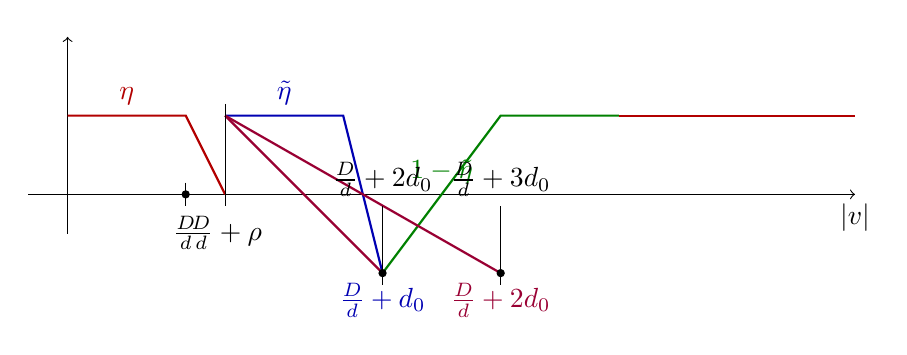
\begin{tikzpicture}
    % Axes
    \draw[->] (-0.5,0) -- (10,0) node[below] {$\vert v \vert$};
    \draw[->] (0,-0.5) -- (0,2) node[left] {};
    
    % Colors
    \colorlet{myred}{red!70!black}
    \colorlet{myblue}{blue!70!black}
    \colorlet{mygreen}{green!50!black}
    \colorlet{mypurple}{purple!80!black}
    
    % Lines
    \draw[myred, thick] (0,1) -- (1.5,1) node[pos=0.5, above] {$\eta$} -- (2,0);
    \draw[myblue, thick] (2,1) -- (3.5,1) node[pos=0.5, above] {$\tilde \eta$} -- (4,-1) node[below] {$\frac{D}{d} + d_0$};
    \draw[mygreen, thick] (4,-1) -- (5.5,1) node[pos=0.5, above] {$1-\tilde \eta$} -- (7,1);
    \draw[myred, thick] (7,1) -- (10,1);
    \draw[mypurple, thick] (2,1) -- (5.5,-1) node[below] {$\frac{D}{d} + 2d_0$};
    \draw[mypurple, thick] (4,-1) -- (2,1);
    
    % Dots
    \fill (1.5,0) circle (1.5pt);
    \fill (4,-1) circle (1.5pt);
    \fill (5.5,-1) circle (1.5pt);
    
    % Labels for axis breakpoints
    \draw (1.5,0.15) -- (1.5,-0.15) node[below] {$\frac{D}{d}$};
    \draw (2,1.15) -- (2,-0.15) node[below] {$\frac{D}{d} + \rho$};
    \draw (4,-1.15) -- (4,-0.15) node[above] {$\frac{D}{d} + 2d_0$};
    \draw (5.5,-1.15) -- (5.5,-0.15) node[above] {$\frac{D}{d} + 3d_0$};
\end{tikzpicture}
\end{document}